\pdfoutput=1

\documentclass{l4proj}

%
% put any packages here
%

\begin{document}
\title{Urban Data Timeline}
\author{Yordan Yordanov}
\date{March 28, 2016}
\maketitle

\begin{abstract}
We show how to produce a level 4 project report using latex and pdflatex using the 
style file l4proj.cls
\end{abstract}

\educationalconsent
%
%NOTE: if you include the educationalconsent (above) and your project is graded an A then
%      it may be entered in the CS Hall of Fame
%
\tableofcontents
%==============================================================================

\chapter{Introduction}
\pagenumbering{arabic}

\section{Background}

Smart cities today represent a perception to integrate both information and communication technologies in an acceptable and maintainable fashion to manage their infrastructure and facilities. The optimal goal is to enhance the quality of life and satisfy the residents’ needs. ICT gives to the people, who maintain these cities, the great opportunity to directly follow what is happening and take actions accordingly. This can be done only by processing the huge amounts of information, collected from sensors, in real time and providing knowledge and information – the keys for discovering inefficiencies. 

However, the biggest asset of a smart city is not the number of cameras or sensors but the people that occupy it. A third of the internet users (Ofcom’s 2015 communications marker report, published on 6 August) represent their smartphone as the most important device for going online. A third of the population owns a smart device and use it every day to bank, shop and access social media. Social media streams, such as Twitter, have a reputation to be extremely useful source of information. Anybody can understand what is happening all around the world in real time. With that comes various opportunities for developers to implement systems that automatically detect and track events as they happen. Smart cities can benefit from that as what better way to improve efficiency than for example identifying and reporting road accidents to the emergency services.

Aiming to help with analyzing these massive amounts of data, the Urban Big Data Centre was established by the UK Economic and Social Research Council to address social, economic and environmental challenges facing cities. Their researchers are undertaking innovative projects, covering topics from big data management to linking and analysing the multi-structural urban data.  Such project is the Integrated Multimedia City Data. 



\subsection{A subsection}

The quick brown fox \cite{fahle} jumped over the lazy dog.
The quick brown fox jumped over the lazy dog.

\chapter{Related Work}
There are applications that have been developed to accomplish similar if not the same goals, but most of them are concentrating on a single data stream. This chapter is presenting a short description of related products, along with key differences and correlations in comparison with the goals of this project.   

\section{The Fox Jumps Over}

The quick brown fox jumped over Uroborus (Figure \ref{uroborus}).


%\vspace{-7mm}
\begin{figure}
\centering
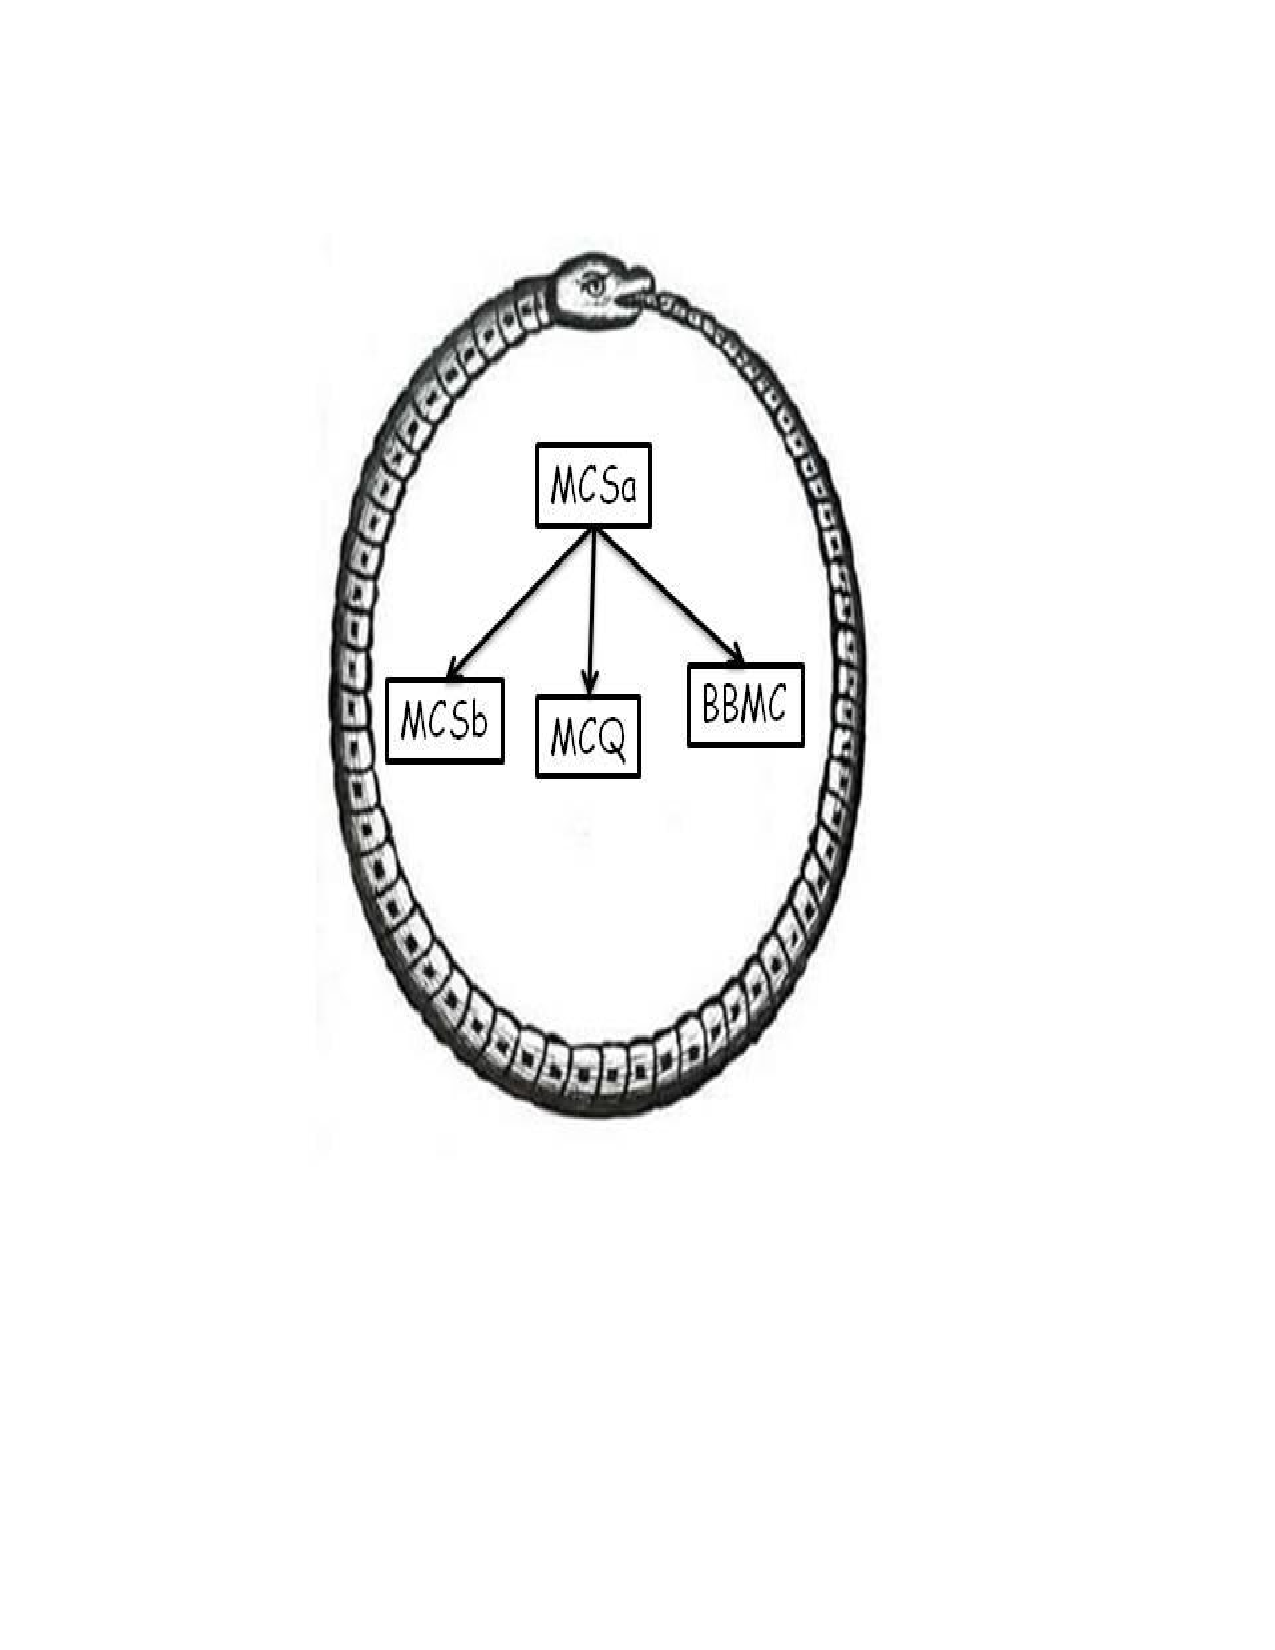
\includegraphics[height=9.2cm,width=13.2cm]{uroboros.pdf}
\vspace{-30mm}
\caption{An alternative hierarchy of the algorithms.}
\label{uroborus}
\end{figure}


The quick brown fox jumped over \cite{ckt} the lazy dog.


\section{The Lazy Dog}

The quick brown fox \cite{am97} jumped over the lazy dog.

\textbf{Google Maps Timeline \cite{GoogleMapsTimeline}}

Google stores a history of where anybody that uses its location services goes. All this data is collected by your device sensors and the navigation you use and then visualized with the Google Maps Timeline feature. It is advertised to be an easy way to view and remember places somebody has been on a given day at a given time. Without any input, the timeline shows predictions of when you have arrived or left a place. One of the key features is highlighting when you have visited the most places and how you had travelled. The application does not offer sharing as Google wants your information to remain private. As far as human interaction goes, you are allowed to correct, confirm or delete a place where Google thinks you had been but even after deleting,  it can still be seen that you had passed by that area. In 2009, the company released a similar feature called Google Latitude that offered sharing of location history but the project was closed down \cite{GMTimeFeature}.


This product has the same initial goal to visualize timely data originating from different streams like navigation history, pictures, travel and walking routes. However what it has in common is it uses a vertical timeline to display the events, it allows searching based on a specific day, month, year and has a way to show (via bar chart) how active you have been every day in the past few weeks. 

\textbf{Social Media Timeline}

All social media websites in the likes of Twitter and Facebook use some sort of a timeline to visualize their user's personal information. However they differ on the way they organize their posts. Facebook describes a timeline to be a place on your profile where you can see your own posts, your friends' activities and stories you're tagged in, sorted by the date and time they were posted. On the other hand, Twitter displays a stream of tweets from accounts that you have chosen to follow. Making use of machine learning algorithms, posts that you are likely to care about more are displayed first.


Despite of the fact that social media applications has as a main goal the delivery of a secure and reliable tool for communication, they also provide their users with the ability to visualize their personal data streams like photos, events, group activities and accomplishments. Both Facebook and Twitter use a vertical timeline and allow for searching based on keywords. One of the key features is infinite scrolling that make the illusion of one endless stream of events by making use of the million users, posting every day. 


\chapter{Solution}
The quick brown fox jumped over the lazy dog.

\section{Choice of technology}

\section{Components communication}

\chapter{Components}

\section{Model}

\section{View}

\section{Controller}

\section{Challenges}

\chapter{Evaluation}

\section{Product evaluation}

\subsection{Initial phase}

\subsection{Final phase}

\section{Testing}

\chapter{Future work}

%%%%%%%%%%%%%%%%
%              %
%  APPENDICES  %
%              %
%%%%%%%%%%%%%%%%
\begin{appendices}

\chapter{Running the Programs}
An example of running from the command line is as follows:
\begin{verbatim}
      > java MaxClique BBMC1 brock200_1.clq 14400
\end{verbatim}
This will apply $BBMC$ with $style = 1$ to the first brock200 DIMACS instance allowing 14400 seconds of cpu time.

\chapter{Generating Random Graphs}
\label{sec:randomGraph}
We generate Erd\'{o}s-R\"{e}nyi random graphs $G(n,p)$ where $n$ is the number of vertices and
each edge is included in the graph with probability $p$ independent from every other edge. It produces
a random graph in DIMACS format with vertices numbered 1 to $n$ inclusive. It can be run from the command line as follows to produce 
a clq file
\begin{verbatim}
      > java RandomGraph 100 0.9 > 100-90-00.clq
\end{verbatim}
\end{appendices}

%%%%%%%%%%%%%%%%%%%%
%   BIBLIOGRAPHY   %
%%%%%%%%%%%%%%%%%%%%

\bibliographystyle{plain}
\bibliography{bib}

\end{document}
